\section{High Class Reference}
\label{classHigh}\index{High@{High}}
{\tt \#include $<$high.h$>$}

Inheritance diagram for High:\begin{figure}[H]
\begin{center}
\leavevmode
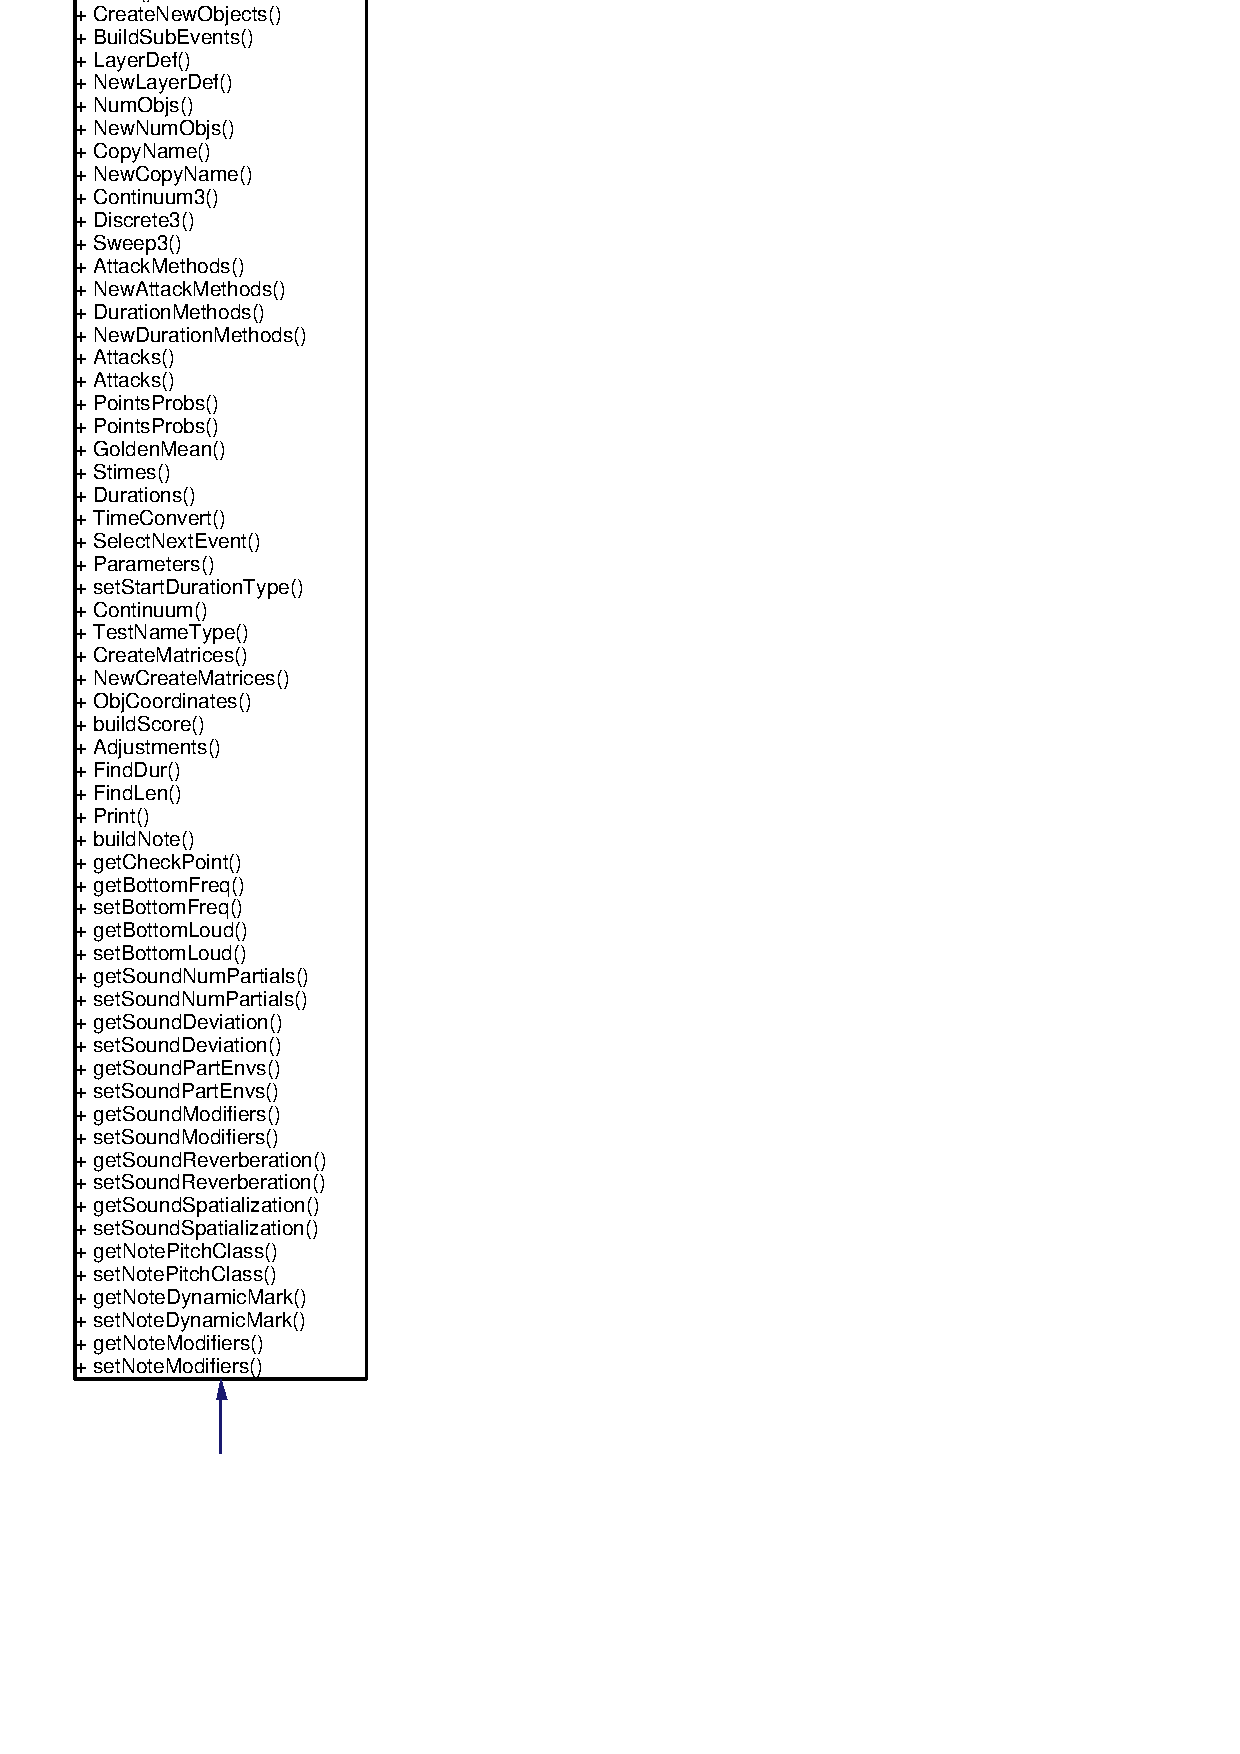
\includegraphics[width=88pt]{classHigh__inherit__graph}
\end{center}
\end{figure}
Collaboration diagram for High:\begin{figure}[H]
\begin{center}
\leavevmode
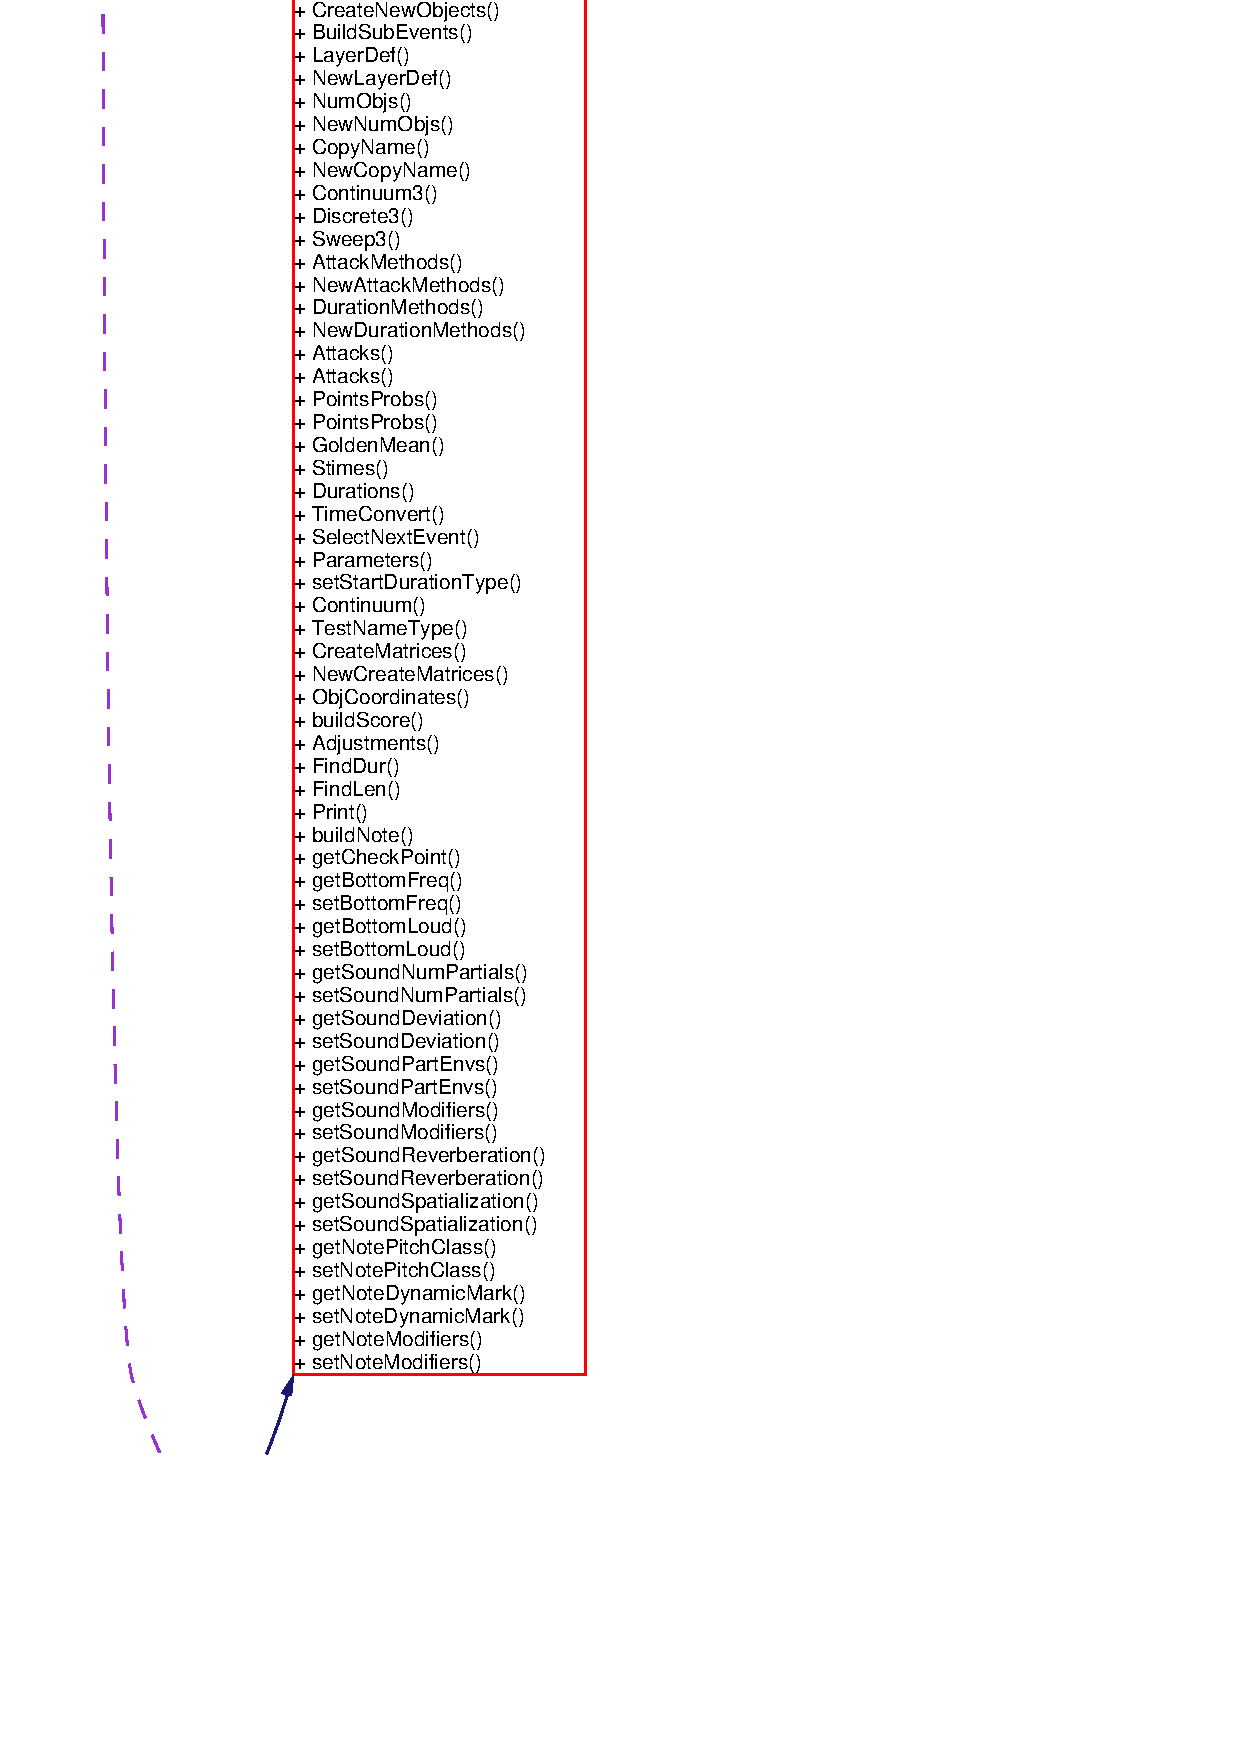
\includegraphics[width=141pt]{classHigh__coll__graph}
\end{center}
\end{figure}
\subsection*{Public Member Functions}
\begin{CompactItemize}
\item 
{\bf High} (float a\-Start\-Time, float a\-Duration, int a\-Type, char $\ast${\bf a\-Name})
\item 
{\bf High} (const  {\bf High} \&orig\-High)
\item 
{\bf $\sim$High} ()
\item 
{\bf High} \& {\bf operator=} (const  {\bf High} \&orig\-High)
\item 
void {\bf clear} ()
\item 
void {\bf Print} ()
\end{CompactItemize}
\subsection*{Protected Attributes}
\begin{CompactItemize}
\item 
double {\bf high\-Density}
\end{CompactItemize}


\subsection{Constructor \& Destructor Documentation}
\index{High@{High}!High@{High}}
\index{High@{High}!High@{High}}
\subsubsection{\setlength{\rightskip}{0pt plus 5cm}High::High (float {\em a\-Start\-Time}, float {\em a\-Duration}, int {\em a\-Type}, char $\ast$ {\em a\-Name})}\label{classHigh_a0}




Definition at line 43 of file high.cpp.

References Event::a\-Name, bottom\-ID, high\-ID, low\-ID, Event::set\-Density(), Event::set\-Duration(), Event::set\-Name(), Event::set\-Start\-Time(), and Event::set\-Type().

Here is the call graph for this function:\begin{figure}[H]
\begin{center}
\leavevmode
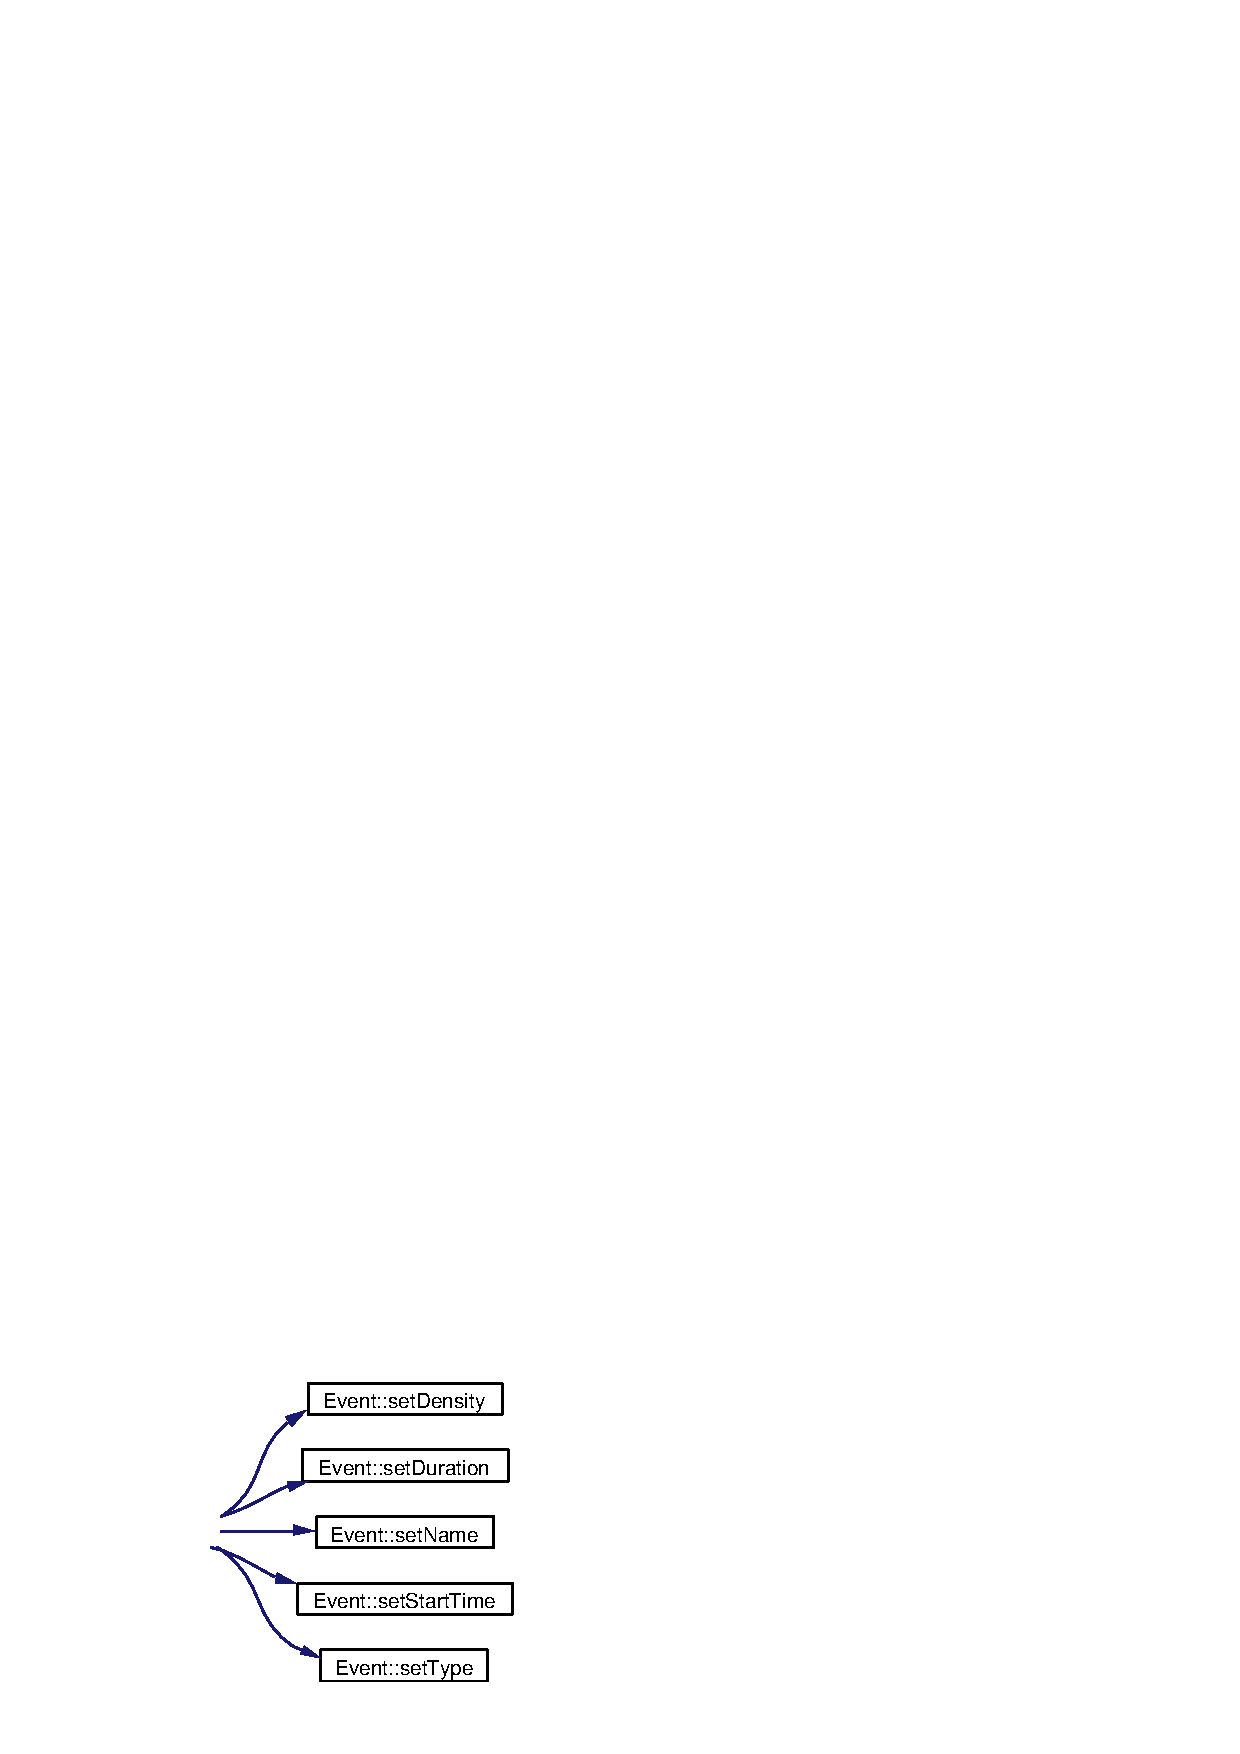
\includegraphics[width=127pt]{classHigh_a0_cgraph}
\end{center}
\end{figure}
\index{High@{High}!High@{High}}
\index{High@{High}!High@{High}}
\subsubsection{\setlength{\rightskip}{0pt plus 5cm}High::High (const {\bf High} \& {\em orig\-High})}\label{classHigh_a1}




Definition at line 77 of file high.cpp.

References bottom\-ID, and high\-ID.\index{High@{High}!~High@{$\sim$High}}
\index{~High@{$\sim$High}!High@{High}}
\subsubsection{\setlength{\rightskip}{0pt plus 5cm}High::$\sim${\bf High} ()}\label{classHigh_a2}




Definition at line 90 of file high.cpp.

\subsection{Member Function Documentation}
\index{High@{High}!clear@{clear}}
\index{clear@{clear}!High@{High}}
\subsubsection{\setlength{\rightskip}{0pt plus 5cm}void High::clear ()\hspace{0.3cm}{\tt  [virtual]}}\label{classHigh_a4}


Clears several internal structures in the {\bf Event}{\rm (p.\,\pageref{classEvent})}: name\-Type, max\-Types, layer\-Dens, objs\-In\-Layer, remain\-Objs, types\-In\-Layer, star\-Tarray, prob\-Sieve\-Array, dur\-Array, prob\-Dur\-Array 

Reimplemented from {\bf Event} {\rm (p.\,\pageref{classEvent_a12})}.

Definition at line 101 of file high.cpp.\index{High@{High}!operator=@{operator=}}
\index{operator=@{operator=}!High@{High}}
\subsubsection{\setlength{\rightskip}{0pt plus 5cm}{\bf High}\& High::operator= (const {\bf High} \& {\em orig\-High})}\label{classHigh_a3}


\index{High@{High}!Print@{Print}}
\index{Print@{Print}!High@{High}}
\subsubsection{\setlength{\rightskip}{0pt plus 5cm}void High::Print ()\hspace{0.3cm}{\tt  [virtual]}}\label{classHigh_a5}




Reimplemented from {\bf Event} {\rm (p.\,\pageref{classEvent_a57})}.

Definition at line 110 of file high.cpp.

References high\-ID, output\-File, Event::the\-Duration, Event::the\-Name, Event::the\-Start\-Time, and Event::u\-Per\-Sec.

\subsection{Member Data Documentation}
\index{High@{High}!highDensity@{highDensity}}
\index{highDensity@{highDensity}!High@{High}}
\subsubsection{\setlength{\rightskip}{0pt plus 5cm}double {\bf High::high\-Density}\hspace{0.3cm}{\tt  [protected]}}\label{classHigh_p0}




Definition at line 37 of file high.h.

The documentation for this class was generated from the following files:\begin{CompactItemize}
\item 
{\bf high.h}\item 
{\bf high.cpp}\end{CompactItemize}
